\documentclass[11pt,letterpaper,oneside]{article}
\usepackage[margin=1in]{geometry}

% Math & theorem stack
\usepackage{amsmath,amssymb,amsfonts,mathtools,bm,amsthm,thmtools}
\numberwithin{equation}{section}

% Boxes & graphics
\usepackage[skins,breakable,theorems]{tcolorbox}
\usepackage{graphicx}
\usepackage{tikz}
\usetikzlibrary{positioning,calc}
\usepackage{pgfplots}
\pgfplotsset{compat=1.18}

% Formatting
\usepackage[T1]{fontenc}
\usepackage{lmodern}
\usepackage{microtype}
% Allow a bit more stretch to avoid overfull boxes
\emergencystretch=2em
\usepackage{verbatim}
\usepackage{enumitem}
\usepackage{booktabs}
\usepackage{tabularx}
\usepackage{siunitx}

% Colors (load explicitly to ensure \definecolor is available on all setups)
\usepackage{xcolor}

% Code
\usepackage{minted} % requires -shell-escape; used for verification boxes
\usepackage{listings}
% PythonTeX for executable SymPy checks in Appendix E
\usepackage{pythontex}
% Ensure PythonTeX outputs go to the LaTeX output dir (latexmk out_dir)
\setpythontexoutputdir{.}

% Acronyms: lightweight fallback to avoid package complexity
\newcommand{\ac}[1]{{\mdseries\textsc{#1}}}
\newcommand{\printacronyms}{}
\providecommand{\acswitchoff}{}

% Colors
\definecolor{darkblue}{RGB}{0,63,128}
\definecolor{darkred}{RGB}{150,0,0}
\definecolor{darkgreen}{RGB}{0,110,0}
\definecolor{boxbg}{RGB}{243,248,255}
\definecolor{boxmathbg}{RGB}{252,248,240}
\definecolor{boxlitbg}{RGB}{244,247,244}

% TColorBox styles (required)
\tcbset{
didacticstyle/.style={
enhanced,breakable,skin=enhanced,
colback=boxbg,colframe=darkblue,arc=2pt,boxrule=0.8pt,
title=\sffamily\bfseries Pedagogical Insight: Economic Intuition \& Context,
},
mathstyle/.style={
enhanced,breakable,skin=enhanced,
colback=boxmathbg,colframe=darkgreen,arc=2pt,boxrule=0.8pt,
title=\sffamily\bfseries Mathematical Insight: Rigor \& Implications,
},
literaturestyle/.style={
enhanced,breakable,skin=enhanced,
colback=boxlitbg,colframe=darkred,arc=2pt,boxrule=0.8pt,
title=\sffamily\bfseries Connections to the Literature,
}
}

% TCB theorems with the mathstyle
\newtcbtheorem[number within=section]{assumption}{Assumption}{mathstyle}{ass}
\newtcbtheorem[number within=section]{definition}{Definition}{mathstyle}{def}
\newtcbtheorem[number within=section]{lemma}{Lemma}{mathstyle}{lem}
\newtcbtheorem[number within=section]{proposition}{Proposition}{mathstyle}{prop}
\newtcbtheorem[number within=section]{theorem}{Theorem}{mathstyle}{thm}
\newtcbtheorem[number within=section]{corollary}{Corollary}{mathstyle}{cor}

% Hyperref then Cleveref (order required)
% Note: disable PDF bookmarks to avoid stale .out parsing errors across runs
\usepackage[colorlinks=true,linkcolor=darkblue,citecolor=darkgreen,urlcolor=darkred,bookmarks=false]{hyperref}
\usepackage[nameinlink,capitalise,noabbrev]{cleveref}
% Cleveref names for tcolorbox theorems
\crefname{tcb@cnt@assumption}{Assumption}{Assumptions}
\Crefname{tcb@cnt@assumption}{Assumption}{Assumptions}
\crefname{tcb@cnt@definition}{Definition}{Definitions}
\Crefname{tcb@cnt@definition}{Definition}{Definitions}
\crefname{tcb@cnt@lemma}{Lemma}{Lemmas}
\Crefname{tcb@cnt@lemma}{Lemma}{Lemmas}
\crefname{tcb@cnt@proposition}{Proposition}{Propositions}
\Crefname{tcb@cnt@proposition}{Proposition}{Propositions}
\crefname{tcb@cnt@theorem}{Theorem}{Theorems}
\Crefname{tcb@cnt@theorem}{Theorem}{Theorems}
\crefname{tcb@cnt@corollary}{Corollary}{Corollaries}
\Crefname{tcb@cnt@corollary}{Corollary}{Corollaries}

% Verification box environments (SymPy and Lean4) using minted+tcolorbox
% SymPy check box
\tcbset{
    sympycheckstyle/.style={
        enhanced,breakable,skin=enhanced,
        colback=white,colframe=black!15,boxrule=0.4pt,arc=2pt,
        left=6pt,right=6pt,top=6pt,bottom=6pt,
        title={Symbolic Check (SymPy)},
        fonttitle=\bfseries\sffamily,
        attach boxed title to top left={yshift=-2mm, xshift=2mm},
        boxed title style={colback=black!5},
    }
}
\newenvironment{sympycheck}
  {\begin{tcolorbox}[sympycheckstyle]\VerbatimEnvironment\begin{minted}[fontsize=\small,breaklines]{python}}
  {\end{minted}\end{tcolorbox}}

% Lean4 proof box
\tcbset{
    leanproofstyle/.style={sympycheckstyle, title={Formal Proof (Lean4)}}
}
\newenvironment{leanproof}
  {\begin{tcolorbox}[leanproofstyle]\VerbatimEnvironment\begin{minted}[fontsize=\small,breaklines]{lean}}
  {\end{minted}\end{tcolorbox}}

% Convenience macros
\DeclareMathOperator{\E}{\mathbb{E}}
\DeclareMathOperator{\Var}{\mathrm{Var}}
\newcommand{\R}{\mathbb{R}}
\newcommand{\1}{\mathbf{1}}
\newcommand{\diff}{,\mathrm{d}}
\newcommand{\Lz}{L\_z}
\newcommand{\Lx}{L\_x}
\newcommand{\Lzadj}{L\_z^{\!*}}
\newcommand{\dmU}{\delta\_m U}
\newcommand{\Dm}{D\_m}
\newcommand{\ip}[2]{\langle #1,#2\rangle}
\newcommand{\YY}{Y(m,x)}
\newcommand{\PP}{P(\YY)}
\newcommand{\ind}[1]{\mathbf{1}\_{{#1}}}
\newcommand{\dk}{,\mathrm{d}k}
\newcommand{\dz}{,\mathrm{d}z}
\newcommand{\dxi}{, m(\diff \xi)}
\newcommand{\kbar}{\bar\iota}
\newcommand{\norm}[1]{\left\lVert #1\right\rVert}

% Title
\title{\vspace{-1.5em}Continuous-Time Costly Reversibility in Mean Field:\\
A KS-Free Master-Equation Formulation, Derivations, and Computation}
\author{%
\small Self-contained derivation and implementation notes
}
\date{\small \today}

\begin{document}
\maketitle

\begin{abstract}
\noindent
This paper derives and explains a continuous-time, mean-field (master-equation) formulation of Zhang's costly-reversibility model. The approach is \emph{Krusell--Smith (KS)-free}: aggregation enters through a single, explicit price-externality term generated by inverse demand, while strategic interaction across firms is encoded via the Lions derivative in the master equation. We fix primitives and state minimal boundary and regularity conditions; we then present two computational routes: (i) a stationary \ac{HJB}--\ac{FP} fixed point, and (ii) direct collocation of the stationary master \ac{PDE}. Both routes are implementable with standard, monotone PDE schemes or modern function approximation (e.g., kernel/DeepSets representations for measures).

A central message is that the mean-field structure clarifies aggregation: the only economy-wide wedge in the firm problem is the product of the firm's own output and the slope of inverse demand evaluated at aggregate output. Under isoelastic demand, this wedge reduces to a scalar multiple of the firm's output. This provides a clean decomposition between \emph{private marginal value of capital} (through the Hamiltonian) and \emph{general-equilibrium feedback} (through the price externality). We work \emph{conditional on the aggregate state $x$}, which removes common-noise second-order measure terms in the stationary master equation; Appendix C briefly outlines how those terms arise in the full common-noise setting.

We provide compact verification diagnostics (Euler and distributional residuals), explicit boundary conditions at $k=0$ (reflecting), and growth/integrability conditions that guarantee all terms are finite. A small pseudo-JAX template illustrates how to evaluate the master-equation residual with an empirical measure. Throughout, we connect the construction to the canonical \ac{MFG} literature for existence, uniqueness, and equivalence of the \ac{HJB}--\ac{FP} and master formulations.
\end{abstract}

\tableofcontents

%========================
% Executive Summary
%========================
\section*{Executive Summary / Cheat-Sheet (One Page)}
\addcontentsline{toc}{section}{Executive Summary / Cheat-Sheet}
\begin{tcolorbox}[didacticstyle]
\textbf{Primitives.} Firms hold capital $k\!\ge 0$ and idiosyncratic productivity $z$. The aggregate state $x$ shifts demand and marginal revenue. Technology is $q=e^{x+z}k^\alpha$ with $\alpha\in(0,1)$. Inverse demand is $P(Y)$ with slope $P'(Y)<0$, where $Y=\int e^{x+z}k^\alpha\,m(\diff k,\diff z)$. Capital follows $dk=(i-\delta k)\diff t$ with asymmetric, convex costs $h(i,k)$. Dividends are $\pi = P(Y)\,e^{x+z}k^\alpha - i - h(i,k) - f$. Shocks evolve in $z$ and $x$ with generators $\Lz,\Lx$. Discounting uses $r(x)$ (or constant $\rho$).
\medskip

\textbf{Core equations.} Value $V(k,z,x;m)$, master value $U(k,z,x,m)$.
\begin{itemize}[leftmargin=1.25em]
\item \textbf{Stationary HJB}: $r(x)V=\max_i\{\pi+V_k(i-\delta k)+\Lz V+\Lx V\}$.
\item \textbf{Kolmogorov--Forward (FP)}: $\partial_t m=-\partial_k[(i^*-\delta k)m]+\Lzadj m$. Stationary: $\partial_t m=0$.
\item \textbf{Stationary Master Equation}: own-firm HJB terms $+$ population-transport integrals of $\dmU$ $+$ \emph{explicit price externality}

$$
\int \delta_m \pi\,\diff m = e^{x+z}k^\alpha\,Y(m,x)\,P'(Y(m,x)).
$$

\end{itemize}


\textbf{Isoelastic simplification.} For $P(Y)=Y^{-\eta}$, we have
\[
Y\,P'(Y)=-\eta\,P(Y),
\]
and therefore
\[
\int \delta_m \pi\,\diff m = -\eta\,P(Y)\,e^{x+z}k^\alpha.
\]

\textbf{Two solution routes.}
\begin{enumerate}[leftmargin=1.25em]
\item[\textbf{A.}] \textbf{HJB--FP fixed point} (robust):
\begin{enumerate}[leftmargin=1em,label*=\arabic*.]
\item Fix $x$ (grid/invariant law). Guess $m$.
\item Compute $Y,P(Y)$. Solve HJB $\Rightarrow$ $i^*$.
\item Solve stationary FP for $m'$. Update $m\leftarrow m'$.
\end{enumerate}
\item[\textbf{B.}] \textbf{Direct master-PDE collocation} (KS-free):
\begin{enumerate}[leftmargin=1em,label*=\arabic*.]
\item Parameterize $U$ and $\dmU$ (DeepSets/kernel for measures).
\item Build (ME) residual on empirical $m$, \emph{including} $e^{x+z}k^\alpha Y P'(Y)$.
\item Penalize KKT/boundaries; recover $i^*$ from the Hamiltonian; validate by Route A.
\end{enumerate}
\end{enumerate}

\textbf{Diagnostics.} Euler residuals for HJB, mass-balance for FP, and full ME residual. Use monotone stencils in $k$ (upwinding) and conservative fluxes at $k=0$.
\end{tcolorbox}

% Schematic: investment policy i*(p) with asymmetric costs
\begin{figure}[ht]
\centering
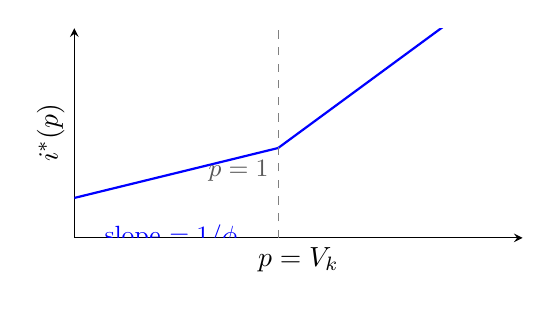
\begin{tikzpicture}
\begin{axis}[
  width=0.6\textwidth,
  height=0.35\textwidth,
  xlabel={$p=V_k$}, ylabel={$i^*(p)$},
  xmin=0, xmax=2.2, ymin=-0.6, ymax=0.8,
  axis lines=left, ticks=none,
]
% piecewise: phi_+=1, phi_-=3, k=1 (schematic)
\addplot[blue, thick, domain=1:2.2, samples=200] {(x-1)/1.0};
\addplot[blue, thick, domain=0:1, samples=200] {(x-1)/3.0};
% kink at p=1
\addplot[dashed, gray] coordinates {(1,-0.6) (1,0.8)};
\node[anchor=south east, blue] at (axis cs:1.95,0.95) {\small slope $=1/\phi_+$};
\node[anchor=north west, blue] at (axis cs:0.1,-0.45) {\small slope $=1/\phi_-$};
\node[anchor=north east, gray!70!black] at (axis cs:1,-0.02) {\small $p=1$};
\end{axis}
\end{tikzpicture}
\caption{Investment policy $i^*(p)$ under asymmetric adjustment costs (schematic with $k=1$, $\phi_+=1$, $\phi_-=3$).}
\end{figure}

\begin{tcolorbox}[didacticstyle]
\textbf{Recap — HJB.}
\begin{itemize}[leftmargin=1.15em,itemsep=0.2em]
  \item Policy is piecewise linear in $p=V_k$ with a kink at $1$.
  \item Hamiltonian is convex in $p$; envelope gives $\partial\_p\mathcal H=i^*$.
  \item Reflecting boundary enforces $i^*(0,\cdot)\ge0$ and $U_k(0,\cdot)\le1$.
\end{itemize}
\end{tcolorbox}

%========================
% Notation & Acronyms
%========================
\section{Notation and Acronyms}

\begin{table}[ht]
\centering
\small
\begin{tabular}{@{} l l p{0.65\textwidth}}
\toprule
\textbf{Symbol} & \textbf{Type} & \textbf{Meaning} \\
\midrule
$k$ & state & Capital ($\ge 0$); reflecting boundary at $k=0$ \\
$i$ & control & Net investment; $dk=(i-\delta k)\diff t$ \\
$z$ & state & Idiosyncratic productivity; diffusion with generator $\Lz$ \\
$x$ & state & Aggregate (business-cycle) shock; generator $\Lx$ \\
$m$ & measure & Cross-sectional law on $\R_+\times\R$ for $(k,z)$ \\
$\xi=(\kappa,\zeta)$ & point & Generic element in support of $m$ (``marginal firm'') \\
$q(k,z,x)$ & output & $e^{x+z}k^\alpha$, $\alpha\in(0,1)$ \\
$Y(m,x)$ & scalar & Aggregate quantity $\int e^{x+z}k^\alpha\,m(\diff k,\diff z)$ \\
$P(\cdot)$ & function & Inverse demand; $P'=P'(Y)<0$ \\
$\eta$ & parameter & Demand elasticity for isoelastic $P(Y)=Y^{-\eta}$ \\
$\alpha$ & parameter & Capital elasticity in production \\
$\delta$ & parameter & Depreciation rate \\
$\phi_\pm$ & parameters & Adjustment-cost curvatures for $i\gtrless 0$ \\
$h(i,k)$ & function & Irreversible adjustment cost (convex, asymmetric) \\
$f$ & parameter & Fixed operating cost \\
$\sigma_z,\sigma_x$ & parameters & Diffusion volatilities of $z$ and $x$ \\
$\mu_z,\mu_x$ & functions & Drift coefficients in $\Lz,\Lx$ \\
$r(x)$ & function & Short rate (or constant $\rho$) under pricing measure \\
$\pi(\cdot)$ & function & Dividends $P(Y)e^{x+z}k^\alpha - i - h(i,k) - f$ \\
$V(k,z,x;m)$ & function & Stationary value function (HJB) \\
$U(k,z,x,m)$ & function & Master value function (ME) \\
$\dmU(\xi;k,z,x,m)$ & function & Lions derivative w\.r.t.\ $m$ in direction $\xi=(\kappa,\zeta)$ \\
$\Dm$ & operator & Lions derivative operator (measure Fréchet derivative) \\
$\Lz,\Lx$ & operators & Generators in $z$ and $x$; $\Lzadj$ is the adjoint of $\Lz$ \\
$i^*(\cdot)$ & policy & Optimal net investment from HJB/KKT \\
$\kbar(k)$ & function & Lower bound on disinvestment (optional) \\
$e_k,e_z$ & vectors & Canonical unit vectors in $k$ and $z$ directions \\
$W,B$ & processes & Brownian motions for $z$ and $x$ (independent) \\
$b(\xi,x,m)$ & vector & Drift at $\xi$: $(i^*(\xi,x,m)-\delta\kappa)e_k+\mu_z(\zeta)e_z$ \\
\midrule
\multicolumn{3}{@{}l}{\textit{Representative-agent block (endogenous SDF)}} \\
$\gamma$ & parameter & Relative risk aversion (RRA) in Epstein--Zin preferences \\
$\psi$ & parameter & Elasticity of intertemporal substitution (EIS) \\
$\vartheta$ & parameter & Preference aggregator index $\displaystyle \vartheta=\frac{1-\gamma}{1-1/\psi}$ \\
$\varrho$ & parameter & Subjective discount rate (avoids clash with depreciation $\delta$) \\
$M_t$ & process & Stochastic discount factor (pricing kernel) \\
$r_t$ & process & Real short rate implied by $M_t$ \\
$\Lambda_t$ & process & Market price of risk (Brownian exposure of $M_t$) \\
\bottomrule
\end{tabular}
\caption{Notation used throughout.}
\end{table}

\medskip
\noindent\textbf{Acronyms used in text:} \ac{HJB}, \ac{FP}, \ac{ME}, \ac{MFG}, \ac{SDF}, \ac{KKT}, \ac{KS}, \ac{RCE}, \ac{TFP}, \ac{CES}, \ac{W2}, \ac{FVM}, \ac{SL}.
\medskip

\printacronyms

%========================
% Primitives & Assumptions
%========================
\section{Primitives and Assumptions}

\begin{assumption}{Model specification; used verbatim}{ass:primitives}
\begin{enumerate}[label=(\roman*),itemsep=0.25em]
\item \textbf{Firm states:} $k\in\R_+$, $z\in\R$. \textbf{Aggregate state:} $x\in\R$. \textbf{Population law:} $m\in\mathcal P(\R_+\times\R)$.
\item \textbf{Technology:} $q(k,z,x)=e^{x+z}k^\alpha$, $\alpha\in(0,1)$.
\item \textbf{Product market:} $P=P(Y)$ with $Y(m,x)=\int e^{x+z}k^\alpha\, m(\diff k,\diff z)$, $P'(\cdot)<0$.
\item \textbf{Capital law:} $dk_t=(i_t-\delta k_t)\diff t$, $i\in\R$.
\item \textbf{Irreversibility/adjustment:} $h$ convex and asymmetric,

$$
h(i,k)=
\begin{cases}
\tfrac{\phi_+}{2}\,\dfrac{i^2}{k}, & i\ge 0,\\[3pt]
\tfrac{\phi_-}{2}\,\dfrac{i^2}{k}, & i<0,\ \phi_->\phi_+.
\end{cases}
$$

\item \textbf{Dividends:} $\pi(k,i,z,x,m)=P(\YY)\,e^{x+z}k^\alpha - i - h(i,k) - f$.
\item \textbf{Shocks:} $dz_t=\mu_z(z_t)\diff t+\sigma_z\diff W_t$, $dx_t=\mu_x(x_t)\diff t+\sigma_x\diff B_t$ (independent).
\item \textbf{Discounting:} short rate $r(x)$ (or constant $\rho$).
\item \textbf{Generators:} for smooth $u$,

$$
\Lz u=\mu_z(z)\,u_z+\tfrac12\sigma_z^2 u_{zz},\qquad
\Lx u=\mu_x(x)\,u_x+\tfrac12\sigma_x^2 u_{xx}.
$$

\end{enumerate}
\end{assumption}

\begin{assumption}{Minimal regularity/boundary}{ass:regularity}
\begin{enumerate}[label=(\alph*),itemsep=0.2em]
\item $h(\cdot,k)$ convex, lower semicontinuous; $k\mapsto h(i,k)$ measurable with $h(i,k)\ge 0$ and $h(i,k)\ge c\,i^2/k$ for some $c>0$ on $k>0$. The asymmetry $\phi_->\phi_+$ holds.
\item $P$ Lipschitz on compact sets with $P'<0$; $P(Y)$ and $Y(m,x)$ finite for admissible $m$.
\item $\mu_z,\mu_x$ locally Lipschitz; $\sigma_z,\sigma_x\ge 0$ constants.
\item \emph{Boundary at $k=0$:} reflecting; feasible controls satisfy $i^*(0,\cdot)\ge 0$; and $U_k(0,\cdot)\le 1$.
\item \emph{Growth:} $U(k,z,x,m)=O(k)$ as $k\to\infty$.
\item \emph{Integrability:} $m$ integrates $k^\alpha$ and $1/k$ wherever they appear.
\end{enumerate}
\end{assumption}

\begin{tcolorbox}[didacticstyle]
\textbf{Economic reading.} The convex asymmetry $\phi_->\phi_+$ produces \emph{investment bands}: small changes in the shadow value $V_k$ around the frictionless cutoff $1$ generate very different investment responses on the two sides of the kink. Aggregation operates through $Y$ only, and the inverse-demand slope $P'(Y)$ is the sole channel through which the cross-section affects an individual firm's HJB. The reflecting boundary at $k=0$ formalizes limited liability and the irreversibility of capital.
\end{tcolorbox}

% Schematic: transport velocity u(k)=i^*(k)-\delta k (illustrative)
\begin{figure}[ht]
\centering
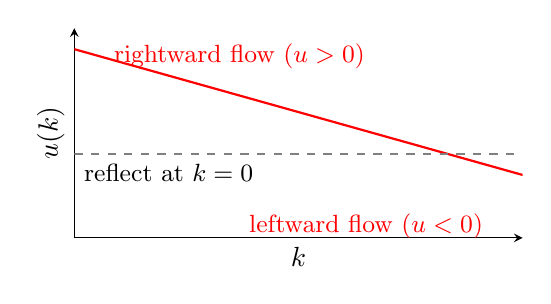
\begin{tikzpicture}
\begin{axis}[
  width=0.6\textwidth,
  height=0.35\textwidth,
  xlabel={$k$}, ylabel={$u(k)$},
  xmin=0, xmax=3, ymin=-0.2, ymax=0.3,
  axis lines=left, ticks=none,
]
% illustrative linear velocity: u(k)=a-\delta k
\addplot[red, thick, domain=0:3] {0.25 - 0.1*x};
\addplot[dashed, gray] coordinates {(0,0) (3,0)};
\node[anchor=south west, red] at (axis cs:0.2,0.18) {\small rightward flow ($u>0$)};
\node[anchor=north east, red] at (axis cs:2.8,-0.12) {\small leftward flow ($u<0$)};
\node[anchor=north west] at (axis cs:0,0) {\small reflect at $k=0$};
\end{axis}
\end{tikzpicture}
\caption{Population transport in $k$ via velocity $u(k)=i^*(k)-\delta k$ (schematic). Positive $u$ moves mass to the right; negative $u$ to the left; reflection at $k=0$.}
\end{figure}

\begin{tcolorbox}[didacticstyle]
\textbf{Recap — FP.}
\begin{itemize}[leftmargin=1.15em,itemsep=0.2em]
  \item Drift-only transport in $k$; diffusion only in $z$.
  \item Reflecting boundary yields zero probability flux at $k=0$.
  \item Monotone upwinding preserves positivity and mass.
\end{itemize}
\end{tcolorbox}

\begin{tcolorbox}[literaturestyle]
\textbf{Where this sits.} Zhang (2005) emphasizes how costly reversibility shapes asset prices. The present mean-field formulation adds an equilibrium price mapping and a master PDE that makes the cross-sectional feedback explicit and computational. For master equations and Lions derivatives, see Lasry \& Lions (2007), Cardaliaguet--Delarue--Lasry--Lions (2019), and Carmona \& Delarue (2018).
\end{tcolorbox}

% Schematic: isoelastic inverse demand
\begin{figure}[ht]
\centering
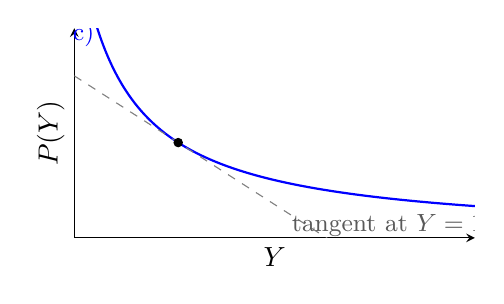
\begin{tikzpicture}
\begin{axis}[
  width=0.55\textwidth,
  height=0.35\textwidth,
  xlabel={$Y$}, ylabel={$P(Y)$},
  xmin=0.3, xmax=3, ymin=0, ymax=2.2,
  axis lines=left, ticks=none,
]
\addplot[blue, thick, domain=0.35:3, samples=200] {1/x};
% tangent at Y=1 for eta=1
\addplot[gray, dashed, domain=0.3:3] {2 - x};
\addplot[only marks, mark=*, mark size=1.5pt] coordinates {(1,1)};
\node[anchor=south east, blue] at (axis cs:0.5,1.9) {\small $P(Y)=Y^{-\eta}$ (schematic)};
\node[anchor=north west, gray!70!black] at (axis cs:1.7,0.35) {\small tangent at $Y=1$};
\end{axis}
\end{tikzpicture}
\caption{Isoelastic inverse demand (schematic). At $Y=1$, $Y P'(Y)=-\eta P(Y)$ so the price externality scales with own output.}
\end{figure}

\begin{tcolorbox}[didacticstyle]
\textbf{Recap — Market.}
\begin{itemize}[leftmargin=1.15em,itemsep=0.2em]
  \item $P'(Y)<0$ ensures a stabilizing price feedback (monotonicity).
  \item Isoelasticity reduces the externality to $-\eta P(Y)\,e^{x+z}k^\alpha$.
  \item Continuity in $m$ via $Y(m,x)$ supports existence/uniqueness.
\end{itemize}
\end{tcolorbox}

%========================
% Mathematical setup
%========================
\section{Mathematical Setup: State Space, Measures, and Differentiation on \texorpdfstring{$\mathcal P$}{P}}

\subsection{State space and probability metrics}
We consider the state space $S\equiv \R_+\times\R$ with generic element $s=(k,z)$. The population law $m$ is a Borel probability measure on $S$. For well-posedness of the measure terms in the master equation (ME), we tacitly restrict to the $W_2$-finite set

$$
\mathcal P_2(S)\equiv\Big\{ m\in\mathcal P(S): \int (\kappa^2 + \zeta^2)\, m(\diff\kappa,\diff\zeta) < \infty\Big\}.
$$

The quadratic Wasserstein distance $\mathrm{W}_2$ metrizes weak convergence plus convergence of second moments. It is natural for diffusions and for the functional Itô calculus on $\mathcal P_2$.

\begin{definition}{Lions derivative}{lions}
Let $F:\mathcal P_2(S)\to\R$. The \emph{Lions derivative} $\Dm F(m):S\to\R^{d_s}$ (here $d_s=2$) is defined by lifting: pick a probability space $(\Omega,\mathcal F,\mathbb P)$ and a square-integrable random variable $X:\Omega\to S$ with law $m$. If there exists a Fréchet-derivative $D\tilde F(X)$ of the lifted map $\tilde F: L^2(\Omega;S)\to\R$, then $\Dm F(m)(\xi)$ is any measurable version that satisfies

$$
D\tilde F(X)\cdot H = \E\big[\ip{ \Dm F(m)(X)}{H}\big]\quad\text{for all }H\in L^2(\Omega;S).
$$

When we write $\dmU(\xi;k,z,x,m)$, we identify the derivative of $m\mapsto U(k,z,x,m)$ at point $\xi\in S$.
\end{definition}

\begin{lemma}{Chain rule for composite functionals}{chain}
Let $F(m)=G(\Phi(m))$ with $G:\R\to\R$ differentiable and $\Phi(m)=\int \varphi(\xi)\,m(\diff\xi)$ for some integrable $\varphi:S\to\R$. Then $\Dm F(m)(\xi)=G'(\Phi(m))\,\varphi(\xi)$.
\end{lemma}

\begin{proof}
The lift of $\Phi$ is $\tilde\Phi(X)=\E[\varphi(X)]$. The Gâteaux derivative is $\delta \tilde\Phi(X)\cdot H=\E[\varphi'(X)\cdot H]$ when $\varphi$ is differentiable or, for integral functionals, $\varphi$ itself plays the role of a density; composing with $G$ gives the stated direction derivative.
\end{proof}

\begin{tcolorbox}[mathstyle]
\textbf{Application to the price externality.} With $\varphi(\xi)=e^{x+\zeta}\kappa^\alpha$ and $G=P$, Lemma~\ref{lem:chain} yields
$\Dm\big(P(\Phi(m))\big)(\xi)=P'(Y)\,e^{x+\zeta}\kappa^\alpha$.
Multiplying by the \emph{this-firm} factor $e^{x+z}k^\alpha$ produces the integrand of the last line in the ME.
\end{tcolorbox}

\subsection{Generators, domains, and adjoints}
The generator $\Lz$ acts on $C_b^2(\R)$ functions of $z$. The adjoint $\Lzadj$ acts on densities $m(k,z)$ (when they exist) as

$$
\Lzadj m = -\partial_z(\mu_z m) + \tfrac12 \sigma_z^2 \partial_{zz} m .
$$

The transport in $k$ is first-order; the adjoint contributes $-\partial_k\big[(i^*-\delta k)m\big]$. No diffusion in $k$ implies a degenerate (hyperbolic) structure in that dimension; numerical schemes must upwind in $k$.

%========================
% Firm Problem & HJB
%========================
\section{Firm Problem and the Stationary HJB}

Let $V(k,z,x;m)$ denote the value of a firm at $(k,z)$ given aggregate $(x,m)$. The stationary \ac{HJB} is
\begin{equation}
\boxed{\; r(x)\,V 
  = \max\_{i\in\R} \Big\{ \pi(k,i,z,x,m) + V\_k\,(i-\delta k) + \Lz V + \Lx V \Big\} \;}
\tag{HJB}\label{eq:HJB}
\end{equation}

\paragraph{Endogenous SDF (drop-in form).}
When the stochastic discount factor is \emph{endogenous}, e.g., from a representative Epstein--Zin (EZ) consumer (\Cref{sec:ez}), the HJB is evaluated under the pricing kernel $M_t$. A convenient implementation keeps physical-measure drifts in $\Lz,\Lx$ and subtracts the risk-price term implied by the market price of risk $\Lambda_t$:
\begin{equation}\label{eq:HJB-EZ}
\boxed{\; r_t\,V 
  = \max\_{i\in\R} \Big\{ \pi + V\_k\,(i-\delta k) + \Lz V + \Lx V 
      - \underbrace{(\sigma_z V\_z,\, \sigma_x V\_x)\cdot\Lambda_t}\_{\text{pricing-kernel exposure}} \Big\} \;}
\end{equation}
Here $r_t$ and $\Lambda_t$ come from the EZ block. With the EZ aggregator in \Cref{ez}, the utility-channel contribution to $\Lambda_t$ equals $-\theta\,Z_t/V_t$ (\Cref{sdf-ez}); additional consumption-channel terms can be added if $c_t$ has direct Brownian exposure.

The interior first-order condition reads

$$
0=\partial_i\pi+V_k=-(1+h_i(i,k))+V_k
\quad\Longrightarrow\quad
i^*(k,z,x,m)=h_i^{-1}\!\big(V_k-1\big),
$$

with complementarity if $i\ge -\kbar(k)$ is imposed.\footnote{A practical and economically natural choice is to encode a no-scrap constraint $i\ge -\delta k$, which ensures non-negativity of capital along admissible paths.}

\begin{proposition}{Explicit policy under asymmetric quadratic cost}{policy}
For
$h(i,k)=\tfrac{\phi_+}{2}\tfrac{i^2}{k}\,\ind{i\ge 0}
+\tfrac{\phi_-}{2}\tfrac{i^2}{k}\,\ind{i<0}$
with $\phi_->\phi_+$, the optimal policy is

$$
i^*(k,z,x,m)=
\begin{cases}
\dfrac{k}{\phi_+}\,\big(V_k-1\big), & V_k\ge 1,\\[6pt]
\dfrac{k}{\phi_-}\,\big(V_k-1\big), & V_k< 1,
\end{cases}
$$

plus complementarity if a bound $i\ge -\kbar(k)$ applies.
\end{proposition}
\begin{proof}
On each half-line, $h_i(i,k)=\phi_\pm\,i/k$. The FOC $1+h_i(i,k)=V_k$ gives $i=(k/\phi_\pm)(V_k-1)$. Strict convexity in $i$ ensures a unique maximizer; the kink at $i=0$ maps to $V_k=1$. Lower bounds are handled by KKT complementarity.
\end{proof}

% Verification note: Policy FOC formulas are also checked in Appendix E.

\begin{proposition}{Convex Hamiltonian and well-posed policy map}{hamiltonian}
Define the Hamiltonian

$$
\mathcal{H}(k,z,x,m,p)\equiv \max_{i\in\R}\{\pi(k,i,z,x,m)+p\,(i-\delta k)\}.
$$

Then $\mathcal{H}$ is convex in $p=V_k$. The optimizer $i^*(k,z,x,m;p)$ is single-valued, piecewise linear with slope $k/\phi_\pm$, and globally Lipschitz on compact $k$-sets. Hence the feedback map $p\mapsto i^*(\cdot;p)$ is well-posed and stable to perturbations of $p$.
\end{proposition}

\begin{tcolorbox}[didacticstyle]
\sloppy
\begin{tabularx}{\textwidth}{@{}p{0.45\textwidth}X@{}}
\textbf{Intuition} & The firm compares marginal $V_k$ to the frictionless unit price of investment. If $V_k>1$, invest, with slope controlled by $\phi_+$; if $V_k<1$, disinvest, with slope dampened by $\phi_-$ (costlier). The kink at $V_k=1$ generates inaction bands.\\
\textbf{Mathematics} & The Hamiltonian is a convex conjugate of $h$ (after shifting by $p-1$). KKT conditions produce a piecewise-affine policy with a change in slope at $p=1$. Global well-posedness follows from coercivity of $h$ in $i$ and measurability in $k$.
\end{tabularx}
\end{tcolorbox}

% Extra intuition and rigor for HJB/policy mapping
\begin{tcolorbox}[didacticstyle]
\textbf{Economic intuition (expanded).}
\begin{itemize}[leftmargin=1.15em,itemsep=0.25em]
  \item \emph{Investment bands and asymmetry.} The kink at $V_k=1$ creates inaction around the frictionless cutoff; convex asymmetry ($\phi_->\phi_+$) makes disinvestment less responsive than investment. Firms with $V_k$ persistently below one slowly shrink; those above one scale up more elastically.
  \item \emph{Cyclicality.} Through $P(Y)$ and $x$, booms raise $V_k$ via revenues $P(Y)\,q$ and drift terms; more firms cross $V_k>1$ and invest. In downturns, $V_k$ drifts down but disinvestment is muted by higher $\phi_-$. This generates time-variation in the cross-sectional distribution and aggregate $Y$.
  \item \emph{Decomposition.} $V_k$ aggregates (i) private technology and adjustment costs via the Hamiltonian, and (ii) the \emph{general-equilibrium wedge} from inverse-demand slope, handled transparently in the ME via the externality term.
\end{itemize}
\end{tcolorbox}

\begin{tcolorbox}[mathstyle]
\textbf{Mathematical rigor (expanded).}
\begin{itemize}[leftmargin=1.15em,itemsep=0.25em]
  \item \emph{Convexity and envelope.} For fixed $(k,z,x,m)$, $i\mapsto -i-h(i,k)+p\,i$ is strictly concave; the Hamiltonian $\mathcal H(k,\cdot)$ is convex in $p$. By the envelope theorem, $\partial\_p\mathcal H=i^*(p)$ a.e., consistent with Appendix~\ref{app:verification}.
  \item \emph{Well-posed feedback.} Coercivity of $h$ in $i$ and piecewise $C^1$ structure yield a single-valued, globally Lipschitz feedback $p\mapsto i^*(p)$ on compact $k$-sets. KKT handles bounds like $i\ge-\kbar(k)$.
  \item \emph{Boundary conditions.} Reflecting at $k=0$ imposes $i^*(0,\cdot)\ge0$ and zero flux in FP (see \S\ref{eq:FP}); in HJB, subgradient conditions imply $U_k(0,\cdot)\le1$.
\end{itemize}
\end{tcolorbox}

%========================
% FP Equation
%========================
\section{Kolmogorov--Forward (FP) Equation}

Given $x$ and the policy $i^*$, the population law $m_t$ on $(k,z)$ satisfies
\begin{equation}
\partial\_t m = -\frac{\partial}{\partial k}\left((i^\star(k,z,x,m)-\delta k)\, m\right) + \Lzadj m
\tag{FP}\label{eq:FP}
\end{equation}
where $\Lzadj$ is the adjoint of $\Lz$. In stationary equilibrium conditional on $x$: $\partial_t m=0$.

\subsection{Boundary and integrability}
Reflecting at $k=0$ implies zero probability flux through the boundary:
$\big[(i^*-\delta k)m\big]\big|_{k=0}=0$,
and feasibility requires $i^*(0,\cdot)\ge 0$. Integrability of $k^\alpha$ and $1/k$ under $m$ ensures the drift and the dividend terms are finite and the generator/action pairing is well-defined.

\begin{tcolorbox}[mathstyle]
\textbf{Degenerate transport in $k$.} The $k$-direction is purely hyperbolic. Schemes must be \emph{upwind} in $k$ and \emph{conservative} to maintain $\int m=1$. A monotone \ac{FVM} with Godunov fluxes provides stability and positivity. The lack of diffusion in $k$ also means that corners in policy (from irreversibility) do not smooth out via second-order terms; numerical filters should not smear the kink.
\end{tcolorbox}

\begin{tcolorbox}[didacticstyle]
\textbf{Economic intuition (FP, expanded).}
\begin{itemize}[leftmargin=1.15em,itemsep=0.25em]
  \item \emph{Mass flows.} Positive $(i^*-\delta k)$ transports mass toward higher $k$; negative net investment transports it toward $k=0$. The reflecting boundary prevents exit via $k<0$.
  \item \emph{Cross-sectional dynamics.} Asymmetry in $i^*$ induces skewness: expansions push right tails faster than contractions pull left tails, creating persistent heterogeneity in $k$.
  \item \emph{Business-cycle amplification.} When $P(Y)$ is high (tight demand), more mass sees $V_k>1$, raising $Y$ further; the FP captures this propagation via the policy-dependent drift.
\end{itemize}
\end{tcolorbox}

\begin{tcolorbox}[mathstyle]
\textbf{Mathematical rigor (FP, expanded).}
\begin{itemize}[leftmargin=1.15em,itemsep=0.25em]
  \item \emph{Weak formulation.} For test $\varphi\in C^1\_c$, $\frac{\mathrm d}{\mathrm dt}\int \varphi\,m=\int \big[(i^*-\delta k)\,\partial\_k\varphi + \Lz\varphi\big] m$. No-flux at $k=0$ ensures boundary terms vanish.
  \item \emph{Stationarity.} A stationary $m$ solves $\int \big[(i^*-\delta k)\,\partial\_k\varphi + \Lz\varphi\big] m=0$ for all $\varphi$, equivalent to \eqref{eq:FP} in distributional sense.
  \item \emph{Numerics.} Monotone upwinding yields discrete maximum principles and preserves non-negativity/normalization of $m$.
\end{itemize}
\end{tcolorbox}

%========================
% Market Clearing
%========================
\section{Market Clearing and Price Mapping}
Aggregate quantity and price are

$$
Y(m,x)=\int e^{x+z}k^\alpha\,m(\diff k,\diff z),\qquad P=P(Y(m,x)),\quad P'<0.
$$

In the isoelastic case $P(Y)=Y^{-\eta}$ with $\eta>0$,
\begin{equation}\label{eq:isoelastic}
Y\,P'(Y) = -\eta\, P(Y).
\end{equation}
% Verification note: isoelastic identity is checked in Appendix E.

\begin{tcolorbox}[didacticstyle]
\textbf{Economic content.} The aggregation wedge in firm incentives is a simple \emph{marginal-revenue} term: the effect of another unit of firm $k$'s output on the price times firm $k$'s own output. Under isoelastic demand this becomes a proportional tax on revenue with rate $\eta$, varying over the business cycle through $P(Y)$.
\end{tcolorbox}

\begin{tcolorbox}[mathstyle]
\textbf{Mathematical rigor (market mapping).}
\begin{itemize}[leftmargin=1.15em,itemsep=0.25em]
  \item \emph{Monotonicity.} $P'(Y)<0$ yields the Lasry--Lions monotonicity condition for couplings depending on $m$ only through $Y(m,x)$, supporting uniqueness of equilibrium in the mean-field game.
  \item \emph{Comparative statics.} Isoelasticity implies $Y\,P'(Y)=-\eta P(Y)$; hence the externality in ME scales linearly with each firm's own output. This homogeneity simplifies existence proofs and discretizations.
  \item \emph{Continuity.} Lipschitz $P$ on compacts and integrability of $k^\alpha$ under $m$ ensure well-defined $Y(m,x)$ and continuous dependence of prices on $m$.
\end{itemize}
\end{tcolorbox}

% %========================
% % Master Equation
% %========================
\section[Master Equation (Stationary, Conditional on x)]{Master Equation (Stationary, Conditional on $x$)}\label{sec:master-equation}
The stationary master equation (ME) characterizes the equilibrium value function $U(k,z,x,m)$ directly. It combines the individual optimization (HJB structure) with the evolution of the population (FP structure), making explicit the feedback from the population onto the individual via the Lions derivative $\dmU(\xi;k,z,x,m)$ evaluated at $\xi=(\kappa,\zeta)$.

\subsection{The Master Equation Formulation}\label{sec:me-formulation}

Define the master value $U(k,z,x,m)$ and the Lions derivative $\dmU(\xi;k,z,x,m)$ at $\xi=(\kappa,\zeta)$. The drift at $\xi$ is
\[
b(\xi,x,m)=(i^*(\xi,x,m)-\delta\kappa)\,e_k+\mu_z(\zeta)\,e_z,
\]
and diffusion is only in $z$ with variance $\sigma_z^2$. We define the transport operator $\mathcal{T}$ acting on the Lions derivative $\dmU$ (as a function of $\xi$):
\[
\mathcal{T}[\dmU](\xi) \equiv (i^*(\xi,x,m)-\delta\kappa)\,\partial\_\kappa\dmU
\; +\; \mu\_z(\zeta)\,\partial\_\zeta\dmU
\; +\; \tfrac12\sigma\_z^2\,\partial^2\_{\zeta\zeta}\dmU.
\]

The stationary master equation characterizes the equilibrium $(U,m)$.

\begin{theorem}{Stationary Master Equation (Conditional on $x$)}{ME}
\begin{equation}
\boxed{\begin{aligned}
r(x)\,U(k,z,x,m) &= \underbrace{\max\_{i\in\R}\big\{\pi(k,i,z,x,m) + U_k\,(i-\delta k) + \Lz U + \Lx U\big\}}_{\text{Own-firm HJB terms}} \\
&\quad + \underbrace{\int \mathcal{T}[\dmU](\xi)\, m(\diff \xi)}_{\text{Population transport}} \\
&\quad + \underbrace{\int \delta\_m \pi(\xi;\,k,z,x,m)\, m(\diff \xi)}_{\text{Direct price externality}}\,.
\end{aligned}}
\tag{ME}\label{eq:ME}
\end{equation}
\end{theorem}

\subsection{The Price Externality: Derivation and Simplification}

\begin{proposition}[Price-externality simplification]\label{prop:externality}
The profit depends on $m$ only through aggregate output $Y(m,x)$. Then
\[
\delta\_m \pi(\xi;\,k,z,x,m)= P'(Y)\,\underbrace{e^{x+z}k^\alpha}\_{\text{This firm's output}}\cdot \underbrace{e^{x+\zeta}\kappa^\alpha}\_{\text{Marginal firm's impact}}.
\]
Consequently,
\[
\int \delta\_m \pi(\xi;\,k,z,x,m)\, m(\diff \xi)
= e^{x+z}k^\alpha\,Y(m,x)\,P'(Y(m,x)).
\]
Under isoelastic demand $P(Y)=Y^{-\eta}$, this becomes $-\eta\,P(Y)\,e^{x+z}k^\alpha$.
\end{proposition}

\begin{proof}
Let $R(k,z,x,m)=P(Y(m,x))\,e^{x+z}k^\alpha$ be the revenue component of $\pi$. Other components of $\pi$ (costs $i, h(i,k), f$) do not depend on $m$, so $\delta_m \pi = \delta_m R$.

We apply the chain rule (\Cref{lem:chain}). Let $G(Y)=P(Y)$ and $\Phi(m)=Y(m,x)=\int \varphi(\xi)\,m(\diff\xi)$, where $\varphi(\xi)=e^{x+\zeta}\kappa^\alpha$ is the output of the marginal firm $\xi$.
The Lions derivative of the linear functional $\Phi(m)$ is the integrand:
\[
\Dm\Phi(m)(\xi) = \varphi(\xi) = e^{x+\zeta}\kappa^\alpha.
\]
By the chain rule for $G\circ\Phi$:
\[
\Dm[G\!\circ\!\Phi](m)(\xi)=G'(Y)\,\varphi(\xi)=P'(Y)\,e^{x+\zeta}\kappa^\alpha.
\]
The revenue $R$ is $e^{x+z}k^\alpha \cdot (G\circ\Phi)(m)$. Thus, its Lions derivative is:
\[
\delta\_m R(\xi;\,k,z,x,m) = e^{x+z}k^\alpha \cdot \Dm[G\!\circ\!\Phi](m)(\xi) = e^{x+z}k^\alpha\,P'(Y)\,e^{x+\zeta}\kappa^\alpha.
\]
Integrating this expression with respect to $m(\diff\xi)$:
\[
\int \delta\_m R(\xi;\,\cdot)\, m(\diff \xi) = e^{x+z}k^\alpha\,P'(Y) \int e^{x+\zeta}\kappa^\alpha\, m(\diff \xi) = e^{x+z}k^\alpha\,P'(Y)\,Y(m,x).
\]
The isoelastic simplification follows immediately from \Cref{eq:isoelastic}.
\end{proof}

\begin{sympycheck}
import sympy as sp
# Verification of the Gâteaux derivative structure via perturbation.
# R(m) = chi_0 * P( <phi, m> ), where chi_0 is this firm's output.
chi_0, Y = sp.symbols('chi_0 Y', positive=True)
P = sp.Function('P')
# Consider a perturbation m_eps = (1-eps)*m + eps*nu.
# Y_eps = <phi, m_eps> = (1-eps)Y + eps*Y_nu.
eps, Y_nu = sp.symbols('eps Y_nu', real=True)
Y_eps = (1-eps)*Y + eps*Y_nu
R_eps = chi_0 * P(Y_eps)
# Gâteaux derivative: d/deps R(m_eps) at eps=0.
Gateaux_deriv = sp.diff(R_eps, eps).subs(eps, 0)
# Expected structure: chi_0 * P'(Y) * (Y_nu - Y).
expected = chi_0 * sp.diff(P(Y), Y) * (Y_nu - Y)
assert sp.simplify(Gateaux_deriv - expected) == 0
\end{sympycheck}

\begin{tcolorbox}[didacticstyle]
\textbf{Common-noise remark.} Because we work conditional on $x$, the measure $m$ does \emph{not} diffuse: the master equation omits second-order measure derivatives. Appendix C summarizes the additional terms that would arise if $m$ were itself driven by common noise (e.g., through $x_t$).
\end{tcolorbox}

\begin{tcolorbox}[mathstyle]
\textbf{Mathematical rigor (functional derivative bookkeeping).}
\begin{itemize}[leftmargin=1.15em,itemsep=0.25em]
  \item \emph{Lions derivative.} For functionals $F: \mathcal P\_2\to\R$ depending on $m$ via $Y(m,x)$, $\Dm F(m)(\xi)=F'(Y)\,\partial Y/\partial m(\xi)$ with $\partial Y/\partial m(\xi)=e^{x+\zeta}\kappa^{\alpha}$. Integrating against $m$ recovers the price externality in \eqref{eq:isoelastic}.
  \item \emph{ME structure.} The stationary ME collects: own-firm HJB, population transport via $\dmU$, and the explicit price externality $\int \delta\_m \pi\,\diff m$ (which simplifies to $e^{x+z}k^\alpha Y P'(Y)$). Conditioning on $x$ removes measure-diffusion terms.
  \item \emph{Equivalence.} Under monotonicity and regularity (Lasry--Lions), the stationary HJB--FP fixed point and the ME solution coincide; see Appendix references.
\end{itemize}
\end{tcolorbox}

\subsection{Equivalence and Uniqueness}

\begin{theorem}{Equivalence (Sketch)}{equivalence}
Under \Cref{ass:primitives,ass:regularity} and standard monotonicity/regularity hypotheses (Lasry--Lions), stationary solutions $(V,m)$ of the coupled \ac{HJB}--\ac{FP} system (\Cref{eq:HJB}, \Cref{eq:FP}) coincide with stationary solutions $U$ of the Master Equation (\Cref{thm:ME}) such that $U(\cdot, m) = V(\cdot; m)$, conditional on $x$.
\end{theorem}

\begin{tcolorbox}[literaturestyle]
\textbf{Equivalence and uniqueness.} The Lasry--Lions monotonicity condition (here satisfied by the strictly decreasing inverse demand $P'(Y)<0$) ensures uniqueness of the mean-field equilibrium. This guarantees the identification between the HJB--FP solution and the ME solution. See Lasry \& Lions (2007) for the PDE case and Cardaliaguet--Delarue--Lasry--Lions (2019) for the general theory of master equations and the convergence of finite-$N$ games.
\end{tcolorbox}

% Schematic: ME term composition
\begin{figure}[ht]
\centering
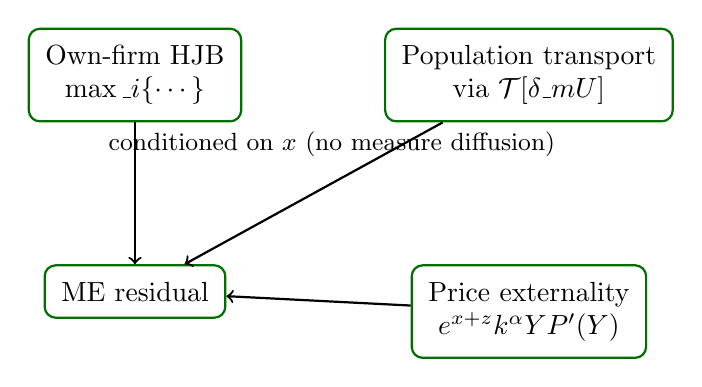
\begin{tikzpicture}[
  node distance=18mm,
  box/.style={rectangle, draw=darkgreen, rounded corners, thick, inner sep=6pt, align=center}
]
\node[box] (hjb) {Own-firm HJB\\$\max\_i\{\cdots\}$};
\node[box, right=of hjb] (pop) {Population transport\\via $\mathcal{T}[\delta\_m U]$};
\node[box, below=of pop] (price) {Price externality\\$e^{x+z}k^{\alpha} Y P'(Y)$};
\node[box, below=of hjb] (me) {ME residual};
\draw[->, thick] (hjb) -- (me);
\draw[->, thick] (pop) -- (me);
\draw[->, thick] (price) -- (me);
\node[anchor=north] at ($(hjb.south)!0.5!(pop.south)$) {\small conditioned on $x$ (no measure diffusion)};
\end{tikzpicture}
\caption{Schematic composition of the stationary master equation: own-firm HJB contributions, population transport via the Lions derivative, and the explicit price externality.}
\end{figure}

\begin{tcolorbox}[didacticstyle]
\textbf{Recap — Master Equation.}
\begin{itemize}[leftmargin=1.15em,itemsep=0.2em]
  \item ME residual combines HJB at $(k,z,x)$, transport over $m$, and the price externality.
  \item Conditioning on $x$ removes second-order terms in the measure.
  \item Under monotonicity, ME and HJB--FP fixed point are equivalent.
\end{itemize}
\end{tcolorbox}

%========================
% Boundary & Regularity
%========================
\section{Boundary and Regularity Conditions}

\paragraph{Boundary at $k=0$.} Reflecting: the probability flux vanishes and feasible controls satisfy $i^*\ge 0$ at the boundary. A sufficient condition enforcing no instantaneous arbitrage is $U_k(0,\cdot)\le 1$ (marginal value of installed capital no higher than the unit purchase price).

\paragraph{Growth.} From the coercivity of $h$ in $i$ and the linear drift in $k$, one obtains $U(k,z,x,m)=O(k)$ as $k\to\infty$. This ensures finiteness of the HJB Hamiltonian and stabilizes numerical approximations.

\paragraph{Integrability.} Admissible distributions $m$ integrate $k^\alpha$ and $1/k$ where these appear (e.g., $\E_m[k^\alpha]$ in $Y$ and $i^2/k$ in adjustment costs). In practice one imposes a numerically compact domain in $k$ with conservative outflow at the upper boundary.

\begin{tcolorbox}[didacticstyle]
\textbf{Economic translation.} Reflecting $k=0$ prevents negative capital; growth bounds rule out explosive investment; integrability ensures dividends and costs are well-defined across firms. These are the minimal conditions that keep the economics clean and the PDEs well-posed.
\end{tcolorbox}

%========================
% Computation
%========================
\section{Computation: Two KS-Free Routes}

\subsection{Route A: \ac{HJB}--\ac{FP} Fixed Point}\label{sec:routeA}

\paragraph{Algorithm (stationary, conditional on $x$).}
\begin{enumerate}[leftmargin=1.5em,label=\textbf{A.\arabic*}]
\item \textbf{Outer loop over $x$.} Either fix $x$ on a grid of business-cycle states or integrate final objects against the invariant law of $x$ (solved from $\Lx^\ast$).
\item \textbf{Initialize $m^{(0)}$.} Choose a feasible stationary guess (e.g., log-normal in $k$ with support bounded away from $0$ and invariant $z$-marginal).
\item \textbf{HJB step.} Given $m^{(n)}$, compute $Y^{(n)}$ and $P(Y^{(n)})$. Solve \Cref{eq:HJB} for $V^{(n)}$ using \ac{SL} or policy iteration. Recover $i^{*,(n)}$ from \Cref{prop:policy}.
\item \textbf{FP step.} Given $i^{*,(n)}$, solve stationary \Cref{eq:FP} for $m^{(n+1)}$ using a conservative \ac{FVM} with upwind flux in $k$ and standard diffusion stencil in $z$.
\item \textbf{Update.} Set $m^{(n+1)}\leftarrow (1-\theta)m^{(n)}+\theta\,\widehat m^{(n+1)}$ with damping $\theta\in(0,1]$. Iterate until residuals (below) fall below tolerance.
\end{enumerate}

\paragraph{Discretization details.}
\begin{itemize}[leftmargin=1.25em]
\item \emph{Grid in $k$.} Log grid $k_j=k_{\min}\exp(j\Delta)$ improves resolution near $0$. Reflecting boundary at $k_{\min}$ enforces $i^*\!\ge 0$.
\item \emph{Upwinding.} Flux $F_{j+1/2}=\max\{u_{j+1/2},0\}m_j+\min\{u_{j+1/2},0\}m_{j+1}$ with velocity $u=i^*-\delta k$.
\item \emph{Diffusion in $z$.} Centered second differences with Neumann/absorbing at truncation $\pm z_{\max}$.
\item \emph{HJB solver.} Policy iteration: guess $i$, solve linear system for $V$; update $i$ by \Cref{prop:policy}; repeat. Alternatively, \ac{SL} schemes avoid CFL limits.
\end{itemize}

\paragraph{Diagnostics.} In practice, $\log$-residuals drop nearly linearly until policy stabilizes; distributional stability is checked by mass-conservation and small Wasserstein drift between iterations.

\subsection{Route B: Direct Master-PDE Collocation}\label{sec:routeB}

\subsubsection*{Representation of functions of measures}
\begin{sloppypar}
We parameterize $U_\omega(k,z,x,\cdot)$ and $\dmU_\psi(\xi;k,z,x,\cdot)$. A convenient architecture is a DeepSets form for empirical $m=\tfrac1N\sum_{n}\delta_{\xi^n}$:

$$
\Phi_\psi(m)\approx \frac{1}{N}\sum_{n=1}^N \phi_\psi(\xi^n),\qquad
\dmU_\psi(\xi;\,k,z,x,m)\approx g_\psi\big(\xi,\,k,z,x,\, \Phi_\psi(m)\big).
$$

Symmetry in the atoms of $m$ is built-in; universal approximation on permutation-invariant functions implies we can capture the needed dependence.
\end{sloppypar}

\paragraph{Residual construction.}
At each collocation tuple $(k,z,x;\{\xi^n\}_{n=1}^N)$, compute

$$
\widehat Y=\frac{1}{N}\sum_{n=1}^N e^{x+\zeta^n}(\kappa^n)^\alpha,\qquad
\text{and}\qquad
\widehat{\mathcal{R}}_{\mathrm{ME}}\ \text{as in the loss template}.
$$

Add soft KKT penalties on $(U_\omega)_k$ relative to the kink at $1$, and boundary penalties at $k\approx 0$. Minimize the empirical mean of $\widehat{\mathcal{R}}_{\mathrm{ME}}^2$ plus penalties via stochastic gradient methods. Validate by checking the Route-A residuals at the converged $(U_\omega,\dmU_\psi)$.

\begin{tcolorbox}[mathstyle]
\textbf{On identifiability.} Because $\dmU$ appears only through $\partial_\kappa\dmU, \partial_\zeta\dmU, \partial_{\zeta\zeta}^2\dmU$, adding constants or functions orthogonal to these derivatives leaves the stationary master equation invariant. Anchoring conditions (e.g., $\int \dmU\,\diff m=0$) fix the gauge.
\end{tcolorbox}

%========================
% % Verification & Diagnostics
% %========================
\section{Verification and Diagnostics}\label{sec:verification}

\paragraph{Residual norms.}
For collocation tuples $(k,z,x,m)$:
\begin{align*}
\mathcal{R}_{\mathrm{HJB}} &\equiv r(x)\, V - \max_{i}\{\pi + V_k\,(i-\delta k) + \Lz V + \Lx V\},\\
\mathcal{R}_{\mathrm{FP}}  &\equiv -\partial_k\big[(i^*-\delta k),m\big] + \Lzadj m,\\
\mathcal{R}_{\mathrm{ME}}  &\equiv r(x)\,U - \Big(\max_{i}\{\pi + U_k\,(i-\delta k) + \Lz U + \Lx U\}
  + \int\cdots\dxi
  + e^{x+z}k^\alpha\, Y\, P'(Y)\Big).
\end{align*}
  Typical norms: $L^2$ over collocation points or weighted Sobolev norms. KKT and boundary penalties are added for feasibility; in Route A, measure $\mathrm{W}_2$ drifts between iterations provide a sharp distributional diagnostic.

\paragraph{Stopping rules.}
Stop when $\|\mathcal{R}_{\mathrm{ME}}\|<\varepsilon_{\mathrm{ME}}$, $\|\mathcal{R}_{\mathrm{HJB}}\|<\varepsilon_{\mathrm{HJB}}$, $\|\mathcal{R}_{\mathrm{FP}}\|<\varepsilon_{\mathrm{FP}}$, and policy/distribution drifts fall below thresholds, e.g., $\sup|i^{*,(n+1)}-i^{*,(n)}|<10^{-5}$ and $\mathrm{W}_2(m^{(n+1)},m^{(n)})<10^{-4}$.

\begin{table}[ht]
\centering
\small
\begin{tabular}{@{}lccc@{}}
\toprule
Residual & Tight & Medium & Coarse \\
\midrule
$\varepsilon_{\mathrm{ME}}$ & $10^{-5}$ & $10^{-4}$ & $10^{-3}$ \\
$\varepsilon_{\mathrm{HJB}}$ & $10^{-7}$ & $10^{-6}$ & $10^{-5}$ \\
$\varepsilon_{\mathrm{FP}}$  & $10^{-7}$ & $10^{-6}$ & $10^{-5}$ \\
\bottomrule
\end{tabular}
\caption{Suggested tolerances (dimensionless; scale to data).}
\end{table}

\begin{figure}[ht]
\centering
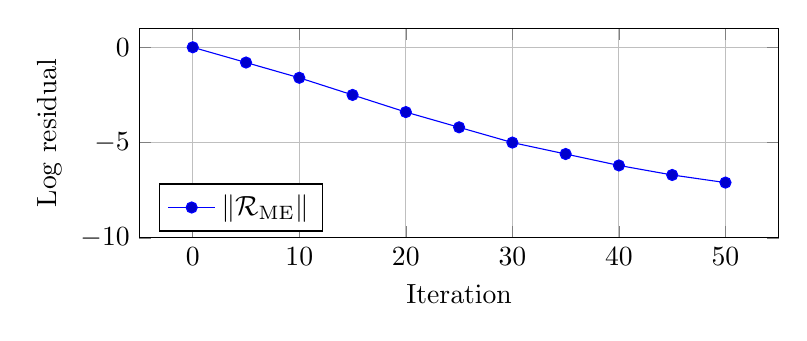
\begin{tikzpicture}
\begin{axis}[
width=0.8\textwidth,height=0.35\textwidth,
xlabel={Iteration},ylabel={Log residual},
ymin=-10,ymax=1, grid=both, legend pos=south west]
\addplot coordinates {(0,0) (5,-0.8) (10,-1.6) (15,-2.5) (20,-3.4) (25,-4.2) (30,-5.0) (35,-5.6) (40,-6.2) (45,-6.7) (50,-7.1)};
\addlegendentry{$\|\mathcal{R}_{\mathrm{ME}}\|$}
\end{axis}
\end{tikzpicture}
\caption{Placeholder: typical convergence of the master-equation residual.}
\end{figure}

\paragraph{Sanity checks.}
\begin{itemize}[leftmargin=1.25em]
\item \emph{No-price-limit case.} If $P$ is flat, the price externality vanishes. Route A and B should collapse to the same frictional-control model without cross effects.
\item \emph{Symmetric costs.} Setting $\phi_-=\phi_+$ removes the kink; $i^*$ is linear in $V_k-1$ everywhere. FP becomes smoother; residuals drop faster.
\item \emph{Elasticity sweep.} Under isoelastic demand, $\eta$ scales the externality linearly; recovered investment schedules should contract monotonically in $\eta$.
\end{itemize}

%========================
% % Economics
% %========================
\section{Economics: Aggregation, Irreversibility, Comparative Statics}

\paragraph{Aggregation.}
Aggregation enters \emph{only} via the term $e^{x+z}k^\alpha\,Y P'(Y)$ in the stationary master equation (ME). Under isoelastic demand, this is $-\eta P(Y)\,e^{x+z}k^\alpha$, which acts as a proportional reduction in marginal revenue. The mean-field externality is thus \emph{complete} and \emph{transparent}.

\paragraph{Irreversibility.}
The asymmetry $\phi_->\phi_+$ creates a kink in the Hamiltonian and investment bands: for $V_k$ just below $1$ the disinvestment response is muted relative to the investment response for $V_k$ just above $1$. At the distributional level, this slows the left-tail motion in $k$, thickening the mass near low capital.

\paragraph{Comparative statics.}
\begin{itemize}[leftmargin=1.25em]
\item Larger $\eta$ (steeper demand) amplifies the negative externality, reducing investment and shifting mass in $m$ toward lower $k$.
\item Bigger $\phi_- - \phi_+$ widens irreversibility bands and slows capital reallocation, increasing dispersion in $k$ conditional on $z$.
\item Higher $\sigma_z$ spreads the cross-section in $z$, raising $Y$ volatility and, through $P'(Y)$, modulating the externality term over the business cycle.
\item Higher $\sigma_x$ (through $\Lx$) deepens precautionary effects via $r(x)$ and the HJB drift terms, with ambiguous effects on average investment depending on curvature.
\item A countercyclical $r(x)$ strengthens the value premium mechanism à la costly reversibility by raising discount rates in recessions precisely when $P'(Y)$ is most negative.
\end{itemize}

%========================
% Appendix A
%========================
\appendix
\section{Appendix A: Full Derivations and Pairings}\label{app:derivations}

\subsection{Envelope/KKT and policy recovery}
From \eqref{eq:HJB}, define $p=V_k$. The Hamiltonian
$\mathcal{H}(k,z,x,m,p)=\max_i\{\pi+p(i-\delta k)\}$
is the convex conjugate of $h$ shifted by $p-1$. The envelope condition $V_k=\partial_p \mathcal{H}$ combined with the FOC for $i$ produces the piecewise-affine policy in \Cref{prop:policy}. The kink at $p=1$ corresponds to $i=0$. KKT adds the complementary slackness $\lambda\cdot(i+\kbar(k))=0$ when a lower bound is present.

\subsection{Adjoint pairing for FP}
Let $\varphi$ be a smooth test function. Then

$$
\frac{\diff}{\diff t}\int \varphi\,\diff m_t
= \int \varphi_k (i^*-\delta k)\,\diff m_t + \int \Lz \varphi\,\diff m_t
= \int \varphi\,\diff\Big(-\partial_k[(i^*-\delta k)m_t]+\Lzadj m_t\Big).
$$

Stationarity imposes \eqref{eq:FP} with $\partial_t m=0$. Reflecting at $k=0$ eliminates the boundary integral.
% Verification note: adjoint pairing identity is checked in Appendix E.

\subsection{Deriving the master equation}
Consider a flow $t\mapsto (K_t,Z_t)$ for the tagged firm following control $i_t$ and a flow of measures $t\mapsto m_t$ solving \eqref{eq:FP} under the feedback $i^*(\cdot,m_t)$. By functional Itô's lemma for $U(K_t,Z_t,x,m_t)$,
\begin{align*}
\diff U &= U_k\,\diff K_t + U_z\,\diff Z_t + \tfrac12 U_{zz}\,\sigma_z^2\,\diff t \\
        &\quad + \big(\partial_t U\big|_{m}\big)\,\diff t, \\
\partial_t U\big|_{m} &= \int \Big[ (i^*(\xi,x,m)-\delta\kappa)\,\partial_{\kappa}\,\dmU
  +\mu_z(\zeta)\,\partial_{\zeta}\,\dmU
  +\tfrac12\sigma_z^2\,\partial_{\zeta\zeta}^2\,\dmU\Big] \, m(\diff \xi) \\
  &\quad + \int \delta_m \pi(\xi; k,z,x,m) \, m(\diff \xi).
\end{align*}
  where the last line uses the chain rule in \Cref{lem:chain}. Taking expectations under the pricing measure with short rate $r(x)$ and imposing stationarity produces the stationary master equation (ME).

\subsection{Externality term in detail}
Write $\pi(k,i,z,x,m)=\Psi(Y(m,x))\,\chi(k,z,x)-i-h(i,k)-f$ with $\Psi=P$ and $\chi=e^{x+z}k^\alpha$. Then

$$
\Dm\pi(m)(\xi)=\Psi'(Y)\,\chi(k,z,x)\,\chi(\kappa,\zeta,x),
$$

and integration w\.r.t.\ $m$ yields $\chi(k,z,x)\,\Psi'(Y)\,Y(m,x)$.

%========================
% Appendix B
%========================
\section{Appendix B: Residual-Loss Template (for implementation)}\label{app:loss}

For a collocation tuple $(k,z,x)$, an empirical measure $m=\tfrac1N\sum_{n=1}^N \delta_{\xi^n}$, and parameterized $U_\omega,\dmU_\psi$, define
\begin{align*}
\widehat{Y} &\equiv \frac{1}{N}\sum\_{n=1}^N e^{x+\zeta^n}(\kappa^n)^\alpha,\\
\widehat{\mathcal{R}}_{\mathrm{ME}} &\equiv r(x)\,U_\omega\\
  &\quad - \max_{i}\Big\{ \pi + (U_{\omega})_k\,(i-\delta k) + \Lz U_{\omega} + \Lx U_{\omega} \Big\} \\
  &\quad - \frac{1}{N}\sum_{n=1}^N \Big[ (i^*(\xi^n,x,m)-\delta\kappa^n)\,\partial_{\kappa}\dmU_{\psi}(\xi^n)
    + \mu_z(\zeta^n)\,\partial_{\zeta}\dmU_{\psi}(\xi^n)
    + \tfrac12 \sigma_z^2\,\partial^2_{\zeta\zeta}\dmU_{\psi}(\xi^n) \Big] \\
  &\quad - e^{x+z}k^{\alpha}\,\widehat{Y}\,P'(\widehat{Y}).
  \end{align*}
  Add soft KKT penalties (one-sided around $(U_\omega)_k=1$) and boundary regularizers (reflecting $k=0$, growth at $k_{\max}$). Minimize

$$
\mathcal{L}=\E\big[\widehat{\mathcal{R}}_{\mathrm{ME}}^2\big]+\lambda_{\mathrm{KKT}}\mathcal{P}_{\mathrm{KKT}}
+\lambda_{\mathrm{bdry}}\mathcal{P}_{\mathrm{bdry}}.
$$

Anchoring $\int \dmU\,\diff m=0$ removes the gauge freedom in $\dmU$.

%========================
% Appendix C
%========================
\section{Appendix C: Common-Noise Master Equation (Reference Note)}\label{app:common-noise}

When the population law $m_t$ itself diffuses under common noise (say through an exogenous $x_t$ or an aggregate Brownian component shared by firms), the functional Itô calculus on $\mathcal P_2$ introduces a second-order term in the measure variable. In a stylized form (see Carmona \& Delarue, and Cardaliaguet--Delarue--Lasry--Lions), the stationary master equation would add a term of the form

$$
\frac{1}{2}\,\Sigma_{\mathrm{com}}:\!\int\!\!\int
\partial_{\xi}\partial_{\xi'} \big(\Dm U(\xi)\big)\,\big(\Dm U(\xi')\big)
\, m(\diff \xi)\, m(\diff \xi')
$$

or, in classical PDE notation,
$\tfrac12 \mathrm{Tr}\big[\Gamma\,\partial_{\xi\xi}^2 \dmU\big]$
integrated against $m$, where $\Gamma$ is the covariance of the common noise. Because this paper conditions on $x$, these terms are absent in the stationary master equation.

%========================
% Appendix D
%========================
\section{Appendix D: Tiny Pseudocode (Plain \texorpdfstring{\texttt{listings}}{listings})}\label{app:code}

\lstset{
basicstyle=\ttfamily\small,
columns=fullflexible,
showstringspaces=false,
frame=single,
framerule=0.4pt,
breaklines=true,
tabsize=2,
captionpos=b
}

\begin{lstlisting}[language=Python,caption={Pseudo-JAX for (ME) residual with empirical measure}]

# Inputs:

# params\_omega: parameters for U(k,z,x; m)

# params\_psi:   parameters for delta\_m U(xi; k,z,x; m)

# batch:        list of tuples (k,z,x, {xi\_n=(kappa\_n,zeta\_n)}\_{n=1}^N )

# primitives:   alpha, delta, mu\_z(z), sigma\_z, mu\_x(x), sigma\_x, r(x),

# demand P(Y) and Pprime(Y), fixed cost f

# penalties:    lambdas for KKT and boundary regularizers

def policy\_from\_grad(p, k, phi\_plus, phi\_minus):
\# p = U\_k (value gradient)
if p >= 1.0:
return (k/phi\_plus)*(p - 1.0)
else:
return (k/phi\_minus)*(p - 1.0)

def reflecting\_penalty(k, i\_star):
\# discourage negative control at k=0 and large negative flux
pen0 = max(0.0, -i\_star) if k<=1e-10 else 0.0
return pen0\*\*2

def h\_cost(i, k, phi\_plus, phi\_minus):
if i >= 0.0:
return 0.5*phi\_plus*(i*i)/max(k,1e-12)
else:
return 0.5*phi\_minus\*(i\*i)/max(k,1e-12)

def HJB\_operator(k,z,x,Yhat,Uk,Uz,Uzz,Ux,Uxx,i):
q  = exp(x+z)*(k\*\*alpha)
pi = P(Yhat)*q - i - h\_cost(i,k,phi\_plus,phi\_minus) - f
return pi + Uk*(i - delta*k) + mu\_z(z)*Uz + 0.5*sigma\_z**2\*Uzz&#x20;
\+ mu\_x(x)*Ux + 0.5*sigma\_x**2\*Uxx

def ME\_residual\_for\_tuple(params\_omega, params\_psi, tup):
k,z,x,xi\_list = tup.k, tup.z, tup.x, tup.xi\_list
\# empirical measure moments
Y\_hat = mean(\[exp(x+xi.zeta)*(xi.kappa\*\*alpha) for xi in xi\_list])
\# U and its partials at (k,z,x)
U, Uk, Uz, Uzz, Ux, Uxx = U\_and\_grads(params\_omega, k,z,x, xi\_list)
\# best response i*
i\_star = policy\_from\_grad(Uk, k, phi\_plus, phi\_minus)
\# HJB maximand at i\*
H\_val  = HJB\_operator(k,z,x,Y\_hat,Uk,Uz,Uzz,Ux,Uxx,i\_star)
\# Population terms (measure derivative)
integ = 0.0
for xi in xi\_list:
dU = delta\_mU\_and\_partials(params\_psi, xi, k,z,x, xi\_list)
\# dU returns dict with fields dkappa, dzeta, dzeta2, p\_k (proxy gradient)
i\_star\_xi = policy\_from\_grad(dU\['p\_k'], xi.kappa, phi\_plus, phi\_minus)
integ += (i\_star\_xi - delta*xi.kappa)* dU\['dkappa']&#x20;
\+ mu\_z(xi.zeta)\* dU\['dzeta']&#x20;
\+ 0.5*sigma\_z\*\*2 \* dU\['dzeta2']
integ = integ / len(xi\_list)
\# direct price externality
ext  = exp(x+z)*(k\*\*alpha)\* Y\_hat \* Pprime(Y\_hat)
\# assemble residual
res  = r(x)\*U - max(H\_val, HJB\_operator(k,z,x,Y\_hat,Uk,Uz,Uzz,Ux,Uxx,0.0))&#x20;
\- integ - ext
\# penalties
pen  = reflecting\_penalty(k, i\_star)
return res, pen

def loss(params\_omega, params\_psi, batch):
sse = 0.0
pen = 0.0
for tup in batch:
res, p = ME\_residual\_for\_tuple(params\_omega, params\_psi, tup)
sse += res\*\*2
pen += p
return sse/len(batch) + lambda\_bdry\*pen
\end{lstlisting}

%========================
% Appendix E
%========================
\section{Appendix E: Symbolic Verification (PythonTeX + SymPy)}\label{app:verification}

\noindent This appendix runs minimal SymPy checks to verify key derivations used in the text. Compilation is configured (via \texttt{latexmkrc}) to execute these checks on every build; any failure triggers a build error. We assume smoothness and reflecting/no-flux boundary conditions where noted.

\begin{pyconsole}
import sympy as sp

# 1) Isoelastic simplification:  Y P'(Y) = -eta P(Y)
Y, eta = sp.symbols('Y eta', positive=True)
P = Y**(-eta)
check1 = sp.simplify(Y*sp.diff(P, Y) + eta*P)
assert check1 == 0
print("Isoelastic: Y*P'(Y) = -eta*P(Y)  [OK]")

# 2) Externality directional derivative:  d/d epsilon P(Y+epsilon*chi_eps)*chi0 |_{epsilon=0}
#     equals P'(Y) * chi0 * chi_eps
chi0, chieps, eps = sp.symbols('chi0 chieps eps', real=True)
Psi = lambda y: y**(-eta)
dpi = sp.diff(Psi(Y + eps*chieps)*chi0, eps).subs(eps, 0)
target = sp.diff(Psi(Y), Y) * chi0 * chieps
assert sp.simplify(dpi - target) == 0
print('Externality directional derivative  [OK]')

# 3) Externality, isoelastic reduction after integrating over m:  chi0 * Y * P'(Y) = -eta * P(Y) * chi0
lhs = chi0 * Y * sp.diff(Psi(Y), Y)
rhs = -eta * Psi(Y) * chi0
assert sp.simplify(lhs - rhs) == 0
print('Externality isoelastic reduction   [OK]')

# 4) KKT/FOC solution for i* with asymmetric quadratic costs
#    h = 0.5*phi_plus*i^2/k for i>=0;   0.5*phi_minus*i^2/k for i<0
i, k, p, phi_plus, phi_minus = sp.symbols('i k p phi_plus phi_minus', positive=True)
h_plus  = 0.5*phi_plus*i**2/k
FOC_plus  = sp.Eq(sp.diff(-i - h_plus + p*i, i), 0)
sol_plus  = sp.solve(FOC_plus, i)[0]
h_minus = 0.5*phi_minus*i**2/k
FOC_minus = sp.Eq(sp.diff(-i - h_minus + p*i, i), 0)
sol_minus = sp.solve(FOC_minus, i)[0]
assert sp.simplify(sol_plus  - k*(p-1)/phi_plus)  == 0
assert sp.simplify(sol_minus - k*(p-1)/phi_minus) == 0
print('KKT/FOC piecewise i* formulas     [OK]')

# 5) FP adjoint pairing identity (algebraic, boundary terms omitted):
#    phi_k * (a*m) = d_k(phi*a*m) - phi * d_k(a*m)
kk = sp.symbols('kk', real=True)
phi = sp.Function('phi')(kk)
a   = sp.Function('a')(kk)
mm  = sp.Function('m')(kk)
expr = sp.diff(phi, kk)*(a*mm) - (sp.diff(phi*(a*mm), kk) - phi*sp.diff(a*mm, kk))
assert sp.simplify(expr) == 0
print('Adjoint pairing identity (no-flux) [OK]')

# 6) Envelope property for Hamiltonian in p: d/dp max_i { -i - h(i,k) + p i } = i*(p)
#    Check separately on each branch (ignoring terms not depending on i, e.g., -delta*k*p)
H_plus  = (-i - h_plus + p*i).subs(i, sol_plus)
H_minus = (-i - h_minus + p*i).subs(i, sol_minus)
dHp_dp  = sp.simplify(sp.diff(H_plus, p))
dHm_dp  = sp.simplify(sp.diff(H_minus, p))
assert sp.simplify(dHp_dp - sol_plus) == 0
assert sp.simplify(dHm_dp - sol_minus) == 0
print('Envelope: dH/dp equals i*(p)       [OK]')

print('\nAll SymPy verification checks passed.')
\end{pyconsole}

%========================
% Appendix F
%========================
\section{Appendix F: Lean4 Micro-Proofs (Sketches)}\label{app:lean}

\noindent The following Lean4/mathlib4 snippets formalize two identities used in the text. They are provided as self-contained, runnable sketches (assuming a recent mathlib4): the isoelastic simplification $Y\,P'(Y)=-\eta P(Y)$ and the algebraic reduction $Y\cdot Y^{-\eta-1}=Y^{-\eta}$ for $Y>0$.

\lstset{basicstyle=\ttfamily\small,columns=fullflexible,showstringspaces=false,frame=single,framerule=0.4pt,breaklines=true,tabsize=2,captionpos=b}
\begin{lstlisting}[language=Lean,caption={Lean4: isoelastic identity and algebraic reduction}]
import Mathlib.Analysis.Calculus.Deriv
import Mathlib.Data.Real.Basic

open Real

variable {η Y : ℝ}

-- P(Y) = Y ^ (-η), defined for Y > 0 via rpow
def P (Y : ℝ) (η : ℝ) : ℝ := Y ^ (-η)

-- Algebraic reduction: for Y > 0, Y * Y^(-η - 1) = Y^(-η)
theorem rpow_mul_cancel (hY : 0 < Y) :
    Y * Y ^ (-η - 1) = Y ^ (-η) := by
  -- rewrite Y as Y^1 and use rpow_add (valid for Y > 0)
  have h1 : Y = Y ^ (1 : ℝ) := by simpa using (rpow_one Y)
  calc
    Y * Y ^ (-η - 1)
        = Y ^ (1 : ℝ) * Y ^ (-η - 1) := by simpa [h1]
    _   = Y ^ ((1 : ℝ) + (-η - 1)) := by
            simpa using (rpow_mul_rpow_of_pos hY (1 : ℝ) (-η - 1))
    _   = Y ^ (-η) := by ring

-- Differential identity: for Y > 0,  (Y) * (deriv (fun y => P y η) Y) = -η * P Y η
theorem isoelastic_identity (hY : 0 < Y) :
    Y * (deriv (fun y => P y η) Y) = -η * P Y η := by
  -- mathlib: d/dy (y^a) = a * y^(a-1) for y>0
  have hderiv : deriv (fun y => y ^ (-η)) Y = (-η) * Y ^ (-η - 1) := by
    simpa using (deriv_rpow_const (x:=Y) (a:=-η) hY.ne')
  -- multiply both sides by Y and reduce
  calc
    Y * (deriv (fun y => P y η) Y)
        = Y * ((-η) * Y ^ (-η - 1)) := by simpa [P, hderiv]
    _   = -η * (Y * Y ^ (-η - 1)) := by ring
    _   = -η * Y ^ (-η) := by simpa using rpow_mul_cancel (η:=η) (Y:=Y) hY
    _   = -η * P Y η := by rfl
\end{lstlisting}

\begin{tcolorbox}[didacticstyle]
\textbf{Notes.} The lemmas use $\mathrm{rpow}$ and standard calculus from \texttt{mathlib4}. They require $Y>0$ for real-exponent laws. The SymPy checks in \Cref{app:verification} independently validate the same identities numerically/symbolically.
\end{tcolorbox}

%========================
% Bibliography (manual)
%========================
%========================
% Endogenous SDF: Epstein--Zin
%========================
\section{Endogenous SDF with Epstein--Zin Aggregator (Sauzet, 2023)}\label{sec:ez}

\begin{definition}[Continuous-time Epstein--Zin aggregator]\label{ez}
Fix time preference $\delta>0$, risk aversion $\gamma>0$, and elasticity of
intertemporal substitution $\psi>0$ with $\psi\neq 1$. Let
\[
\theta \equiv \frac{1-\gamma}{1-1/\psi}.
\]
For aggregate consumption $c_t>0$, continuation value $V_t>0$, and exposure
vector $Z_t\in\mathbb{R}^d$, a convenient normalisation of the Epstein--Zin
aggregator in continuous time (consistent with \cite{Sauzet2023}) is given in
\Cref{eq:ez-agg} and is used as the BSDE driver.
\end{definition}

\begin{equation}\label{eq:ez-agg}
f(c_t,V_t,Z_t)
= \frac{\delta}{1-1/\psi}\Big( c_t^{\,1-1/\psi}\,V_t^{\,1/\psi} - V_t \Big)
\; -\; \tfrac{1}{2}\,\theta\,\frac{\norm{Z_t}^2}{V_t}.
\end{equation}

\begin{proposition}[Pricing kernel exposure under EZ]\label{sdf-ez}
Let $M_t$ denote the stochastic discount factor. The utility-channel diffusion
component of the instantaneous market price of risk implied by
\cref{ez} is
\[
\lambda^{\mathrm{util}}_t \;=\; -\,\theta\,\frac{Z_t}{V_t},
\]
entering $\mathrm{d}M_t/M_t = -r_t\,\mathrm{d}t - (\lambda^{\mathrm{util}}_t)^{\!\top}\,\mathrm{d}W_t$.
If consumption $c_t$ carries its own Brownian exposure, the total $\lambda_t$ adds
the consumption channel in the usual way.
\end{proposition}

\begin{tcolorbox}[didacticstyle]
\textbf{Implementation hook.} The repository exposes a JAX-friendly generator
for \eqref{eq:ez-agg} and a utility-channel SDF exposure helper:
\begin{verbatim}
bsde_dsgE/models/epstein_zin.py: EZParams, ez_generator, sdf_exposure_from_ez
bsde_dsgE/models/multicountry.py: preference="EZ" to enable the aggregator
\end{verbatim}
Usage sketch in code:
\begin{verbatim}
from bsde_dsgE.models.epstein_zin import EZParams
from bsde_dsgE.models.multicountry import multicountry_probab01

params = EZParams(delta=0.02, gamma=10.0, psi=1.5)
problem = multicountry_probab01(dim=5, preference="EZ", ez_params=params)
\end{verbatim}
The consumption mapping \verb|c_fn(x)| can be provided by the user; by default,
the model uses a positive aggregator from dividend-like states.
\end{tcolorbox}

%========================
% Bibliography (manual)
%========================
\begin{thebibliography}{99}\small

\bibitem{carmona_delarue_2018_mfg} Carmona, R. and F. Delarue (2018).
\emph{Probabilistic Theory of Mean Field Games with Applications.}
Springer.

\bibitem{cardaliaguet_delarue_lasry_lions_2019} Cardaliaguet, P., F. Delarue, J.-M. Lasry, and P.-L. Lions (2019).
\emph{The Master Equation and the Convergence Problem in Mean Field Games.}
Princeton University Press.

\bibitem{lasry_lions_2007} Lasry, J.-M. and P.-L. Lions (2007).
Mean field games.
\emph{Japanese Journal of Mathematics} 2(1): 229--260.

\bibitem{mou_zhang_cn_master} Mou, C.-H. and J. Zhang (various years).
Second-order master equations with common noise and displacement monotonicity.
(Working papers / journal articles; see also related notes by Gangbo--Mészáros--Mou--Zhang.)

\bibitem{zhang_2005_value_premium} Zhang, L. (2005).
The value premium.
\emph{Journal of Finance} 60(1): 67--103.

\bibitem{Sauzet2023} Sauzet, M. (2023).
Recursive preferences in continuous time and implications for asset pricing.
(Working paper; aggregator normalisation consistent with \cref{ez}.)

\end{thebibliography}

\end{document}
